\documentclass{article}
\usepackage{graphicx}
\usepackage{float}
\usepackage[utf8]{inputenc}
\usepackage{csquotes}
\usepackage[backend=biber,style=numeric,natbib=true,sorting=none]{biblatex}
\usepackage[colorlinks=true,linkcolor=blue,citecolor=blue,urlcolor=blue]{hyperref}
\usepackage{cleveref}
\addbibresource{main.bib}

\title{IQL: Research project. Temporal Evolution of Word Order}
\author{Jairo El Yazidi Ríos, Virginia Nicosia \\
https://github.com/JairoRY/Evolution-of-Word-Order}
\date{June 2025}

\begin{document}

\maketitle

\section{Introduction}

The order of words is one of the core features of the syntactic structure in natural languages; it reflects both the grammatical and pragmatic properties of a language. In the case of English, the dominant word order today is Subject-Verb-Object (SVO), but historical evidence suggests that earlier stages of English permitted a greater degree of variation using often also  the Subject-Object-Verb (SOV) and Verb-Subject-Object (VSO) patterns. This study investigates whether the distribution of basic word order patterns in English has changed over time and to what extent such changes can be detected in syntactically annotated corpora.

We examined and compared two parsed corpora of English from different historical periods: the Parsed Corpus of Early English Correspondence 2 (PCEEC2) \cite{PCEEC2} and the SUSANNE corpus \cite{SUSANNE}; by analyzing the frequency and types of basic word orders present in these corpora, we aim to identify potential diachronic shifts and assess the stability or evolution of syntactic patterns in English.

\section{Results}

\begin{table}[H]
    \centering
    \label{tab:susanne}
    \begin{tabular}{lrrr}
        \hline
        Word Order & Count & Percent (\%) \\
        \hline
        SVO & 3,828 & 91.06 \\
SOV & 3 & 0.07 \\
VSO & 117 & 2.78 \\
VOS & 108 & 2.57 \\
OSV & 24 & 0.57 \\
OVS & 124 & 2.95 \\
\textbf{TOTAL} & \textbf{4,204} & \textbf{100}\\
\hline
    \end{tabular}
    \caption{Word Order Statistics in Modern English}
\end{table}

\begin{table}[H]
    \centering
    \label{tab:pceec}
    \begin{tabular}{lrrr}
        \hline
        Word Order & Count & Percent (\%) \\
        \hline
        SVO & 15,871 & 52.85 \\
SOV & 1,220 & 4.06 \\
VSO & 5,693 & 18.96 \\
VOS & 6,141 & 20.45 \\
OSV & 427 & 1.42 \\
OVS & 678 & 2.26 \\
\textbf{TOTAL} & \textbf{30,030} & \textbf{100}\\
\hline

    \end{tabular}
    \caption{Word Order Statistics in Early English}
\end{table}

\begin{figure}[H]
    \centering
    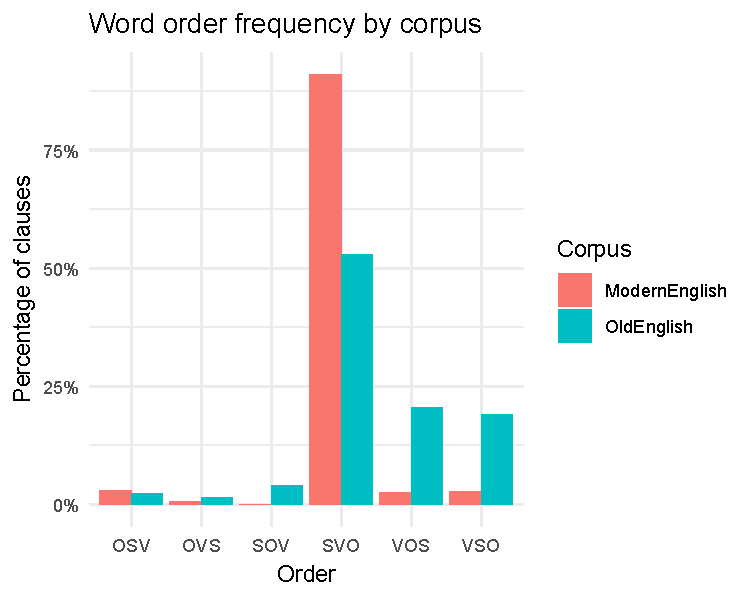
\includegraphics[width=0.8\linewidth]{bar_word_order}
    \caption{Distribution of word order patterns (bar chart)}
    \label{fig:bar_word_order}
\end{figure}

\begin{figure}[H]
    \centering
    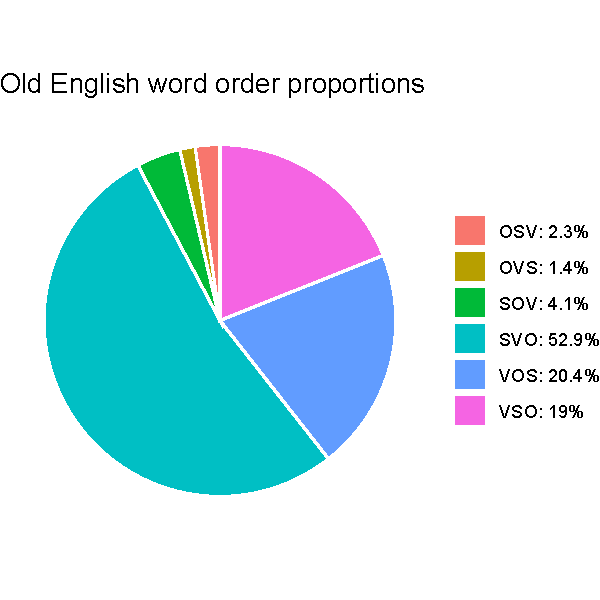
\includegraphics[width=0.6\linewidth]{pie_old_english}
    \caption{Word order distribution in Old English (pie chart)}
    \label{fig:pie_old_english}
\end{figure}

\begin{figure}[H]
    \centering
    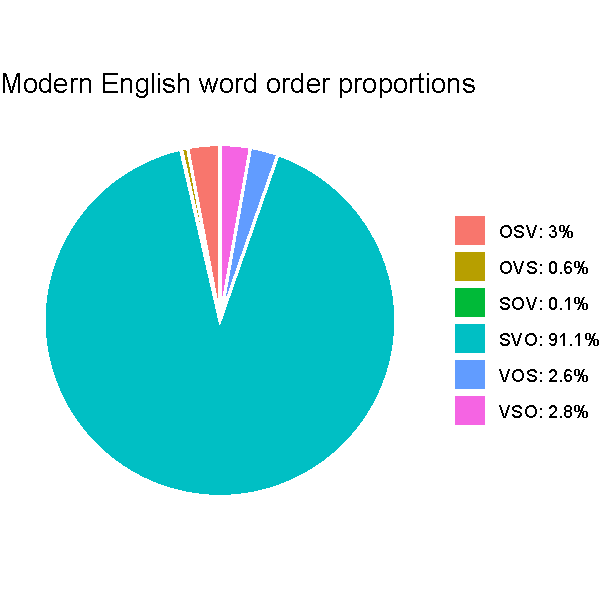
\includegraphics[width=0.6\linewidth]{pie_modern_english}
    \caption{Word order distribution in Modern English (pie chart)}
    \label{fig:pie_modern_english}
\end{figure}

\section{Discussion}

Comparative analysis of word-order patterns between the PCEEC2 and SUSANNE corpora reveals a significant diachronic shift in the syntactic structure of English: the clearest trend is the increased dominance of the SVO (Subject-Verb-Object) order in the modern language, where it accounts for more than 91\% of the observed clauses. This is in stark contrast to the earlier English corpus, where the SVO constitutes only about 53\% of the data, with a notably more diverse distribution among the other word orders.

In Early English correspondence from the 15\textsuperscript{th} to 17\textsuperscript{th} centuries, the relatively low proportion of SVO and the substantial presence of VSO (19\%) and VOS (20\%) suggest that English syntax at the time was still in flux; these alternative word orders may reflect syntactic variability driven by information structure, topicalization, or residual verb initial patterns inherited from earlier stages of English but also the stylistic conventions specific to epistolary texts, such as fronting constituents for emphasis, might have contributed to this distribution.

The representative of standard written British English from the 20\textsuperscript{th} century shows a strong convergence toward a fixed SVO order; the almost total dominance of SVO here is consistent with the well documented syntactic stabilization of Modern English. The decline in the constructions of VSO and VOS (both below 3\%) indicates a loss of flexibility in the structure of the clause and an increasing dependence on the order of the constituents to mark the grammatical function, as the morphological cues become less obvious.

Other non canonical orders, such as OSV, OVS, and SOV remain marginal in both corpora although their combined presence is somewhat more notable in earlier stages of the language; this may reflect constructions such as topicalization or embedded clause structures that become rarer or more rigidly marked in contemporary English.

In general, these findings support the hypothesis of a gradual but clear transition to strict SVO word order in English: this aligns with historical syntactic studies \cite{Fischer1988} that describe a shift from the relatively freer word order of Old and Middle English toward the configurational syntax characteristic of Present Day English. The shift is also indicative of a broader trend toward analytic structure and reduced reliance on inflectional morphology, with word order taking on greater grammatical significance.

These results also highlight the importance of considering corpus composition and text type: PCEEC2, which is composed of personal letters, may reflect more informal and variable usage, while SUSANNE, drawn from edited written sources, represents a more formal and standardized register. The stylistic variation was not controlled for in this study but it is worth noting that genre and register probably interact with syntactic variability.

\section{Methods}

The central research question that guides this study is the following: \textbf{Has the predominant word order in English changed over time and, if so, how?} Our goal is to detect shifts in the frequency of the six logically possible basic word orders (SVO, SOV, VSO, VOS, OVS and OSV) by comparing historical and modern parsed corpora.

To address this question, we selected two syntactically annotated corpora:

\begin{itemize}
    \item \textbf{PCEEC2} (Parsed Corpus of Early English Correspondence 2): This corpus contains personal correspondence texts from the 15\textsuperscript{th} to the late 17\textsuperscript{th} centuries. It is manually annotated and provides rich syntactic information for historical English.
    \item \textbf{SUSANNE} Corpus: A modern corpus derived from a selection of texts in the Brown Corpus. It is fully parsed and represents the contemporary (20\textsuperscript{th} century) English usage.
\end{itemize}

Before we decided to work with these corpora, we conducted an initial phase of research to evaluate potential resources. We identified several high-quality candidates \cite{Taylor2020} that covered all the time periods that we originally wanted to study, including the \textbf{YCOE} (York-Toronto-Helsinki Parsed Corpus of Old English) \cite{YCOE}, \textbf{PPCME2} (Penn-Helsinki Parsed Corpus of Middle English 2) \cite{PPCME2}, \textbf{PPCEME} (Penn-Helsinki Parsed Corpus of Early Modern English) \cite{PPCEME} and \textbf{PPCMBE2} (Penn Parsed Corpus of Modern British English 2) \cite{PPCMBE2}. However, despite repeated efforts, we found that these corpora were not freely available for academic use without a paid license, which made them unsuitable for the open-access requirement of our project.

We also experimented with an intermediate corpus, the \textbf{Royal Society Corpus} \cite{RSCorpus}, which contains scientific writing from the 17\textsuperscript{th} to 19\textsuperscript{th} centuries, approximately bridging the temporal gap between the PCEEC2 and SUSANNE corpora. Unfortunately, this corpus was only partially tagged and did not provide full syntactic parsing. Its annotation relied on Penn Treebank style part-of-speech (POS) tagging, which, while useful for identifying individual word classes, does not offer syntactic constituent structure or grammatical function labels such as subject or object. This limitation also meant that we could not reliably identify clause boundaries or distinguish between main and subordinate clauses, particularly in cases involving relative clauses. As a result, the Royal Society Corpus was excluded from the quantitative analysis.

In our final analysis, we made the methodological decision to ignore the stylistic differences between texts because, for example, PCEEC2 consists primarily of personal letters, while SUSANNE includes a variety of genres, such as academic and formal writing. Although stylistic variation may influence sentence structure and word order, our focus was on overall trends in syntactic configurations over time rather than genre-specific language use.

Due to the structural and tagset differences between the PCEEC2 and SUSANNE corpora, we developed two separate processing scripts, one for each corpus, since although both corpora are fully parsed, they use distinct annotation conventions, tree structures, and file formats. Our scripts were customized to handle the specific format of each corpus, parse trees, and syntactic labeling, enabling us to extract subject-verb-object relations and classify each sentence into one of the six basic word order types.

By combining careful corpus selection, custom processing scripts, and consistent criteria for word order classification, we aimed to provide a robust comparison of word order distribution in historical and modern English.

\section{Conclusion}

The findings of our study support the hypothesis that English has undergone a substantial reconfiguration in its dominant word order over time, culminating in the overwhelmingly SVO-dominant structure of Present-Day English. Our analysis of the PCEEC2 corpus, which covers earlier stages of the language, reveals a more heterogeneous distribution of word orders: although SVO is already the most frequent pattern in PCEEC2, a significant proportion of sentences follow alternative orders, particularly VSO and VOS. This diversity reflects the relatively flexible syntax of earlier English, in which word order was more sensitive to discourse factors, information structure, and syntactic constructions.

In radical contrast, the SUSANNE corpus, which represents contemporary English, exhibits a clear dominance of the SVO word order (over 91\%), with all other configurations occurring at negligible frequencies, and strongly suggests that the development towards a fixed SVO order has solidified.

Together, these results illustrate a diachronic trend from syntactic flexibility to configurational rigidity. The data align with previous linguistic accounts of the evolution of English word order, and they provide empirical corpus-based confirmation of the syntactic restructuring processes that have shaped the language from its historical stages to the present day.

\printbibliography

\end{document}
